\documentclass[11pt]{exam}
\usepackage[margin=1in]{geometry}
\pagestyle{plain}
\usepackage{amsmath,amsfonts,amssymb,amsthm,enumerate}
\usepackage{multicol}
\usepackage[]{graphicx}
\usepackage{hyperref}
\usepackage{tikz}
\usepackage{pgfplots}
\usepackage{subfigure}
\usepackage[final]{pdfpages}

\addtolength{\footskip}{2\baselineskip} % to lower the page numbers
\title{\vspace{-0.5in} Math 115 \\ Worksheet Section 3.2}
\date{}


% \theoremstyle{definition}
% \newtheorem{problem}{Problem}
\renewcommand{\questionlabel}{\textbf{Problem~\thequestion.}}
%\printanswers

\begin{document}
\maketitle
\vspace{-0.75in}
\section*{Warm-up question}

\noindent
$\left( e^x \right)' =$ \fillin[\(e^x\)] $\left( a^x \right)' =$
\fillin[\( a^x\ln(a)\)] $\left( \sin(x) \right)' =$ \fillin[\(\cos(x)\)] $\left( \cos(x) \right)' =$\fillin[\(-\sin(x)\)]

\noindent


\vspace{2em}
\begin{questions}
  \question An animal population is given by \(P(t) = 300(1.044)^t\)
    where \(t\) is the number of years since the study of the
    population began. Find \(P'(5)\) and provide a practical
    interpretation of your result.
    \begin{solution}
      \(P'(x) = 300(1.044)^t \ln(1.044)\) so \(P'(5) = 300(1.044)^5
      \ln(1.044) \approx 16.02\). This means that from \(5\) years to
      \(5\) years and \(1\) month after the study began, the animal
      population will increase by approximately
      \(\frac{300}{12}(1.044)^5\ln(1.044)\) animals. (This is about
      \(1.39\) animals).
    \end{solution}
    \vspace{1em}
  \question Find the quadratic polynomial \(g(x) = ax^2+bx+c\) which
    best fits the function \(f(x) = e^x\) at \(x=0\), in the sense
    that \[
      g(0) = f(0) \text{ and }g'(0) = f'(0)\text{ and }g''(0) = f''(0)
    \]
    Using a computer or calculator, sketch the graphs of \(f\) and
    \(g\) on the same axes. What do you notice?
    \begin{solution}
      We know that \(f'(x) = e^x\) and \(f''(x) = e^x\), so
      \(f(0)=f'(0)=f''(0)=1\). We compute
      \begin{align*}
        g(x) = ax^2+bx+c & \implies g(0)=c\\
        g'(x) = 2ax+b & \implies g'(0) = b\\
        g''(x) = 2a & \implies g''(0) = 2a
      \end{align*}
      Thus, \(g(x) = \frac{1}{2}x^2+x+1\) is the quadratic polynomial
      that best fits the function \(f(x) = e^x\) at \(x=0\). Below,
      \(e^x\) is in red and \(g(x)\) is in blue.
      \begin{center}
        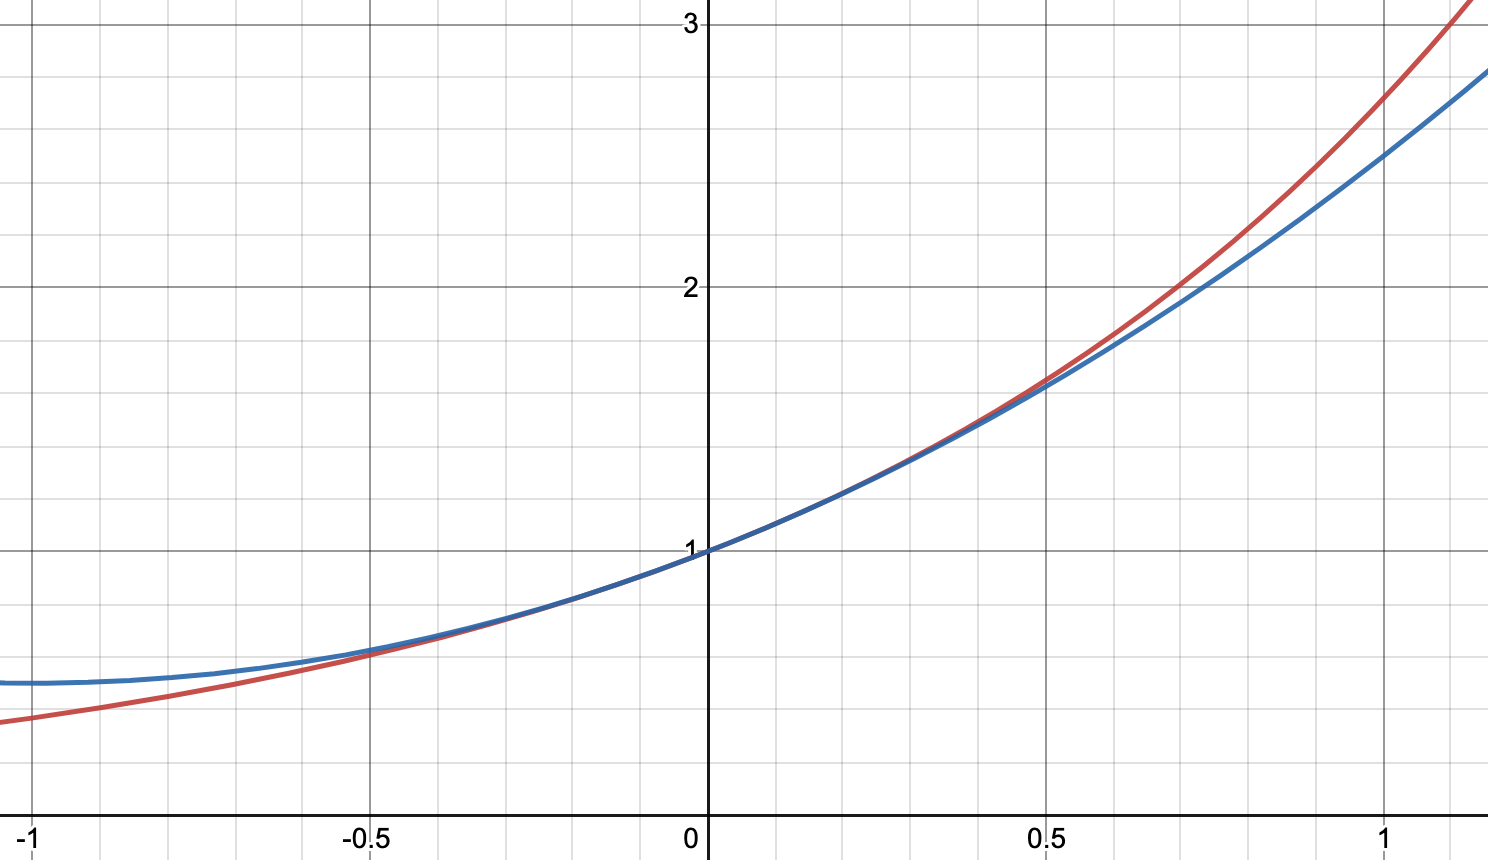
\includegraphics[scale=0.4]{Figures/ex_vs_approx}
      \end{center}
    \end{solution}
    \vspace{1em}
  \question Using the equation of the tangent line to the graph of $e^x$ at $x=0$, show that $$e^x\geq 1+x$$ for all values of $x$.  A sketch may be helpful.
    \begin{solution}
      If \(f(x) = e^x\), then \(f'(x) = e^x\), so the tangent line for
      \(e^x\) at \(x=0\) has slope \(f'(0) = e^0 = 1\) and passes
      through the point \((0,1)\). Thus, the tangent line has equation
      \(y = x+1\). Furthermore, \(e^x\) is concave up since \(f''(x) =
      e^x > 0\) for all values of \(x\). Thus, the graph of \(e^x\)
      lies above its tangent line at \(x=0\) and, since \(e^x\) is
      always increasing, it will never cross back down to intersect
      the tangent line \(y=x+1\).
    \end{solution}
    \vspace{1em}
  \question Find the $50^{\text{th}}$ derivative of $y = \cos(x)$.
    \begin{solution}
      We know that
      \begin{align*}
        y' & = -\sin(x)\\
        y'' & = -\cos(x)\\
        y''' & = \sin(x)\\
        y^{(4)} & = \cos(x)
      \end{align*}
      So, by this pattern, \(y^{(4n)} = \cos(x)\) for any positive
      integer \(n\). Therefore, \(y^{(48)} = \cos(x)\) and \(y^{(50)}
      = y^{(2)} = -\cos(x)\).
    \end{solution}
    \vspace{1em}
  \question Find the tangent lines to $f(x)=\sin(x)$ at $x=\frac{4\pi}{3}$  and at $x=\frac{10\pi}{3}$.  Graph them, along with $\sin(x)$.  What do you notice?  Express the second as a transformation of the first.
    \begin{solution}
      We know that \(f'(x) = \cos(x)\), so \(f'\left( \frac{4\pi}{3}
      \right) = \cos\left(\frac{4\pi}{3}\right) =
      -\frac{1}{2}\). The tangent line at \(x=\frac{4\pi}{3}\) also
      passes through \((\frac{4\pi}{3}, \frac{\sqrt{3}}{2})\) since
      \(\sin\left(\frac{4\pi}{3}\right) = -\frac{\sqrt{3}}{2}\). Thus, the
      tangent line of \(\sin(x)\) at \(x = \frac{4\pi}{3}\) is \[
        l_1(x) = -\frac{1}{2}\left(x-\frac{4\pi}{3}\right)-\frac{\sqrt{3}}{2}
      \]
      Similarly, we check \(f'\left( \frac{10\pi}{3} \right) = \cos\left(\frac{10\pi}{3}\right) =
      \frac{1}{2}\) and \(f\left( \frac{10\pi}{3} \right) =
      -\frac{\sqrt{3}}{2}\) and so the tangent line at
      \(x=\frac{10\pi}{3}\) is given by \[
        l_2(x) = -\frac{1}{2}\left(x-\frac{10\pi}{3}\right)-\frac{\sqrt{3}}{2}
      \]
      Thus, these two lines are just horizontal translations of each
      other: \(l_2(x) = l_1(x-2\pi)\).
    \end{solution}
    \vspace{1em}
  \question Are the following statements true or false? Give an explanation for your answer.
\begin{enumerate}[(a)]
	\item If $f(x)$ is increasing, then $f'(x)$ is increasing.
	\item There is no function such that $f'(x) = f(x)$ for all $x$ besides the constant function $f(x)=0$.
	\item There is no function such that $f'(x) = -f(x)$ for all $x$ besides the constant function $f(x)=0$.
	\item There is no function such that $f''(x) = -f(x)$ for all $x$ besides the constant function $f(x)=0$.
	\item If $f(x)$ is defined for all $x$, then $f'(x)$ is defined for all $x$.
\end{enumerate}
\begin{solution}
  \begin{enumerate}
  \item False. Consider \(f(x)=x^3\) on \((-\infty,0)\).
  \item False. For \(f(x) = e^x\), \(f'(x) = e^x\).
  \item False. Consider \(f(x) = (e^{-1})^x = e^{-x}\). Then, \(f'(x)
    = \ln(e^{-1}) (e^{-1})^x = - e^{-x}\).
  \item False. Consider \(f(x) = \sin(x)\). Then, \(f''(x) = -\sin(x)\).
  \item False. Consider \(f(x) = |x|\). Then, \(f'(0)\) is undefined.
  \end{enumerate}
\end{solution}
  \question For what value(s) of $a$ are $y = a^x$ and $y=x+1$ tangent at $x=0$?
    \begin{solution}
      We check \(y'(x) = \ln(a) a^x\) so \(y'(0) = \ln(a) a^0 =
      \ln(a)\). Thus, \(\ln(a) = 1\) can only be satisfied by
      \(a=e\). 
    \end{solution}
    \pagebreak
  \question (Winter 2017 Exam 3) %p9
    A Math 115 coordinator is trying to create functions with certain properties in
order to test students’ understanding of various calculus
concepts. She wants a function \(f(x)\) of the form \[
  f(x) =
  \begin{cases}
    ax^2 + ax + be^x & \text{ for }x<0\\
    a+2\cos(x) & \text{ for }x \geq 0
  \end{cases}
\]
  where \(a\) and \(b\) are constants. Find all value(s) of \(a\) and \(b\) for which \(f(x)\) be differentiable at \(x = 0\). Show enough work
to justify your answer.
\begin{solution}
  See part (a) of \href{https://dhsp.math.lsa.umich.edu/exams/115exam3/w17/s9.pdf}{https://dhsp.math.lsa.umich.edu/exams/115exam3/w17/s9.pdf}
\end{solution}
\vspace{1in}
\question Explain for which values of $a>0$ the function $a^x$ is
  increasing and for which values it is decreasing. Is this consistent
  with your formula for \((a^x)'\)?
  \begin{solution}
    We know we get exponential growth for \(a > 1\) and exponential
    decay for \(0 < a < 1\). If we set \(f(x) = a^x\) and compute
    \(f'(x) = \ln(a) a^x\), we notice that \(a^x > 0\) for all
    \(a>0\) and for all \(x\),
    so we just have to figure out the sign of \(\ln(a)\). If \(0 < a <
    1\), then \(\ln(a) < 0\) and if \(a > 1\), then \(\ln(a) > 0\). 
    Therefore, this is consistent since \(f'(x) > 0\) when \(a>1\) and
    \(f'(x) < 0\) when \(0 < a < 1\).
  \end{solution}
  \vspace{0.5in}
\question Give an example of:
\begin{enumerate}[(a)]
\item An exponential function for which the derivative is always negative. 
\item A function $f$ such that $f'''(x)=f(x)$. 
\end{enumerate}
\begin{solution}
  \begin{enumerate}[(a)]
  \item As discussed in the previous problem, any function
    \(f(x) = a^x\) for \(0 < a < 1\) will work. So,
    \(f(x) = \left( \frac{1}{2} \right)^x\) works.
  \item Of course, \(f(x) = 0\) will work, as will \(f(x) = e^x\).
  \end{enumerate}
\end{solution}
\vspace{0.5in}
\question In 2009, the population of Mexico was 111 million and
  growing $1.13\%$ annually, while the population of the US was 307
  million and growing $0.975\%$ annually. If we measure growth rates
  in people/year, which population was growing faster in 2009? Note
  \(\ln(1.0113) \approx 0.01124\) and \(\ln(1.00975) \approx 0.009702\).
  \begin{solution}
    Let \(M(t) = 111(1.0113)^t\) be the population of Mexico in
    millions for \(t\) the number of years after 2009. Let \(U(t) =
    307(1.00975)^t\) be the population of the United States in
    millions for \(t\) the number of years after 2009. We compute \[
      M'(t) =  111 \ln(1.0133) (1.0113)^t \implies M'(0) = 111
      \ln(1.0113) \approx 111(0.01124) = 1.24764
    \]
    and \[
      U'(t) = 307 \ln(1.009702) (1.009702)^t \implies U'(0) = 307
      \ln(1.009702) \approx 307(0.009702) = 2.978514
    \]
    Thus, the population of the USA was growing faster in 2009.
  \end{solution}
\end{questions}
\end{document}
%%% Local Variables:
%%% mode: latex
%%% TeX-master: t
%%% End:
